\section{Auswertung}
\label{sec:Auswertung}
  \subsection{Berechnung der Winkelrichtgröße $D$}
  Zur Bestimmung der Winkelrichtgröße $D$ wurde die Kraft $F$ in Abhängigkeit des Auslenkungswinkels $\varphi$ bei festem Abstand von 
  $0,19975 [\unit{\meter}]$ gemessen. Diese Werte sind in Tabelle (\ref{tab:F_von_phi}) zu sehen. Die Winkelrichtgröße $D$ wird durch Gleichung 
  (\ref{eqn:Winkelrichtgröße}) bestimmt und ist ebenfalls in Tabelle (\ref{tab:F_von_phi}) eingetragen, dort auf vier Nachkommastellen gerundet.
   Das gemittelte Ergebnis ist 
  $\bar{D} = (21,0 \pm 0,8) \cdot 10^{-3} \left[\unit{\newton\meter} \right]$.
  
  \begin{table}[H]
    \centering 
    \caption{Kraft in Abhängigkeit vom Auslenkungswinkel}
    \label{tab:F_von_phi}
    \begin{tblr}{colspec={c c c}}
        \toprule
        $\varphi [^{\circ}]$ & F [\unit{\newton}] & D [\unit{\newton\meter}]\\
        \midrule
        20 & 0,026 & 0,0149\\
        30 & 0,050 & 0,0191\\
        40 & 0,068 & 0,0195\\  
        50 & 0,090 & 0,0206\\
        60 & 0,120 & 0,0229\\
        70 & 0,136 & 0,0222\\
        80 & 0,156 & 0,0223\\
        90 & 0,184 & 0,0234\\
        100 & 0,20 & 0,0229\\
        110 & 0,21 & 0,0218\\
        \bottomrule
    \end{tblr}
  \end{table}
  

  \subsection{Berechnung des Eigenträgheitmoments}
  Um das Eigenträgheitsmoment der Drillachse $I_{\text{Drill}}$ zu bestimmen, wurde die fünffache Periodendauer $T$ in Abhängigkeit vom Abstand $a$
  bei einer Auslenkung von $90 ^{\circ}$ gemessen. Diese Messwerte sind in Tabelle (\ref{tab:Bestimmung_I_D}) vermerkt. 
  \begin{table}[H]
    \centering 
    \caption{Fünffache Periodendauer in Abhängigkeit vom Abstand}
    \label{tab:Bestimmung_I_D}
    \begin{tblr}{colspec={c c}}
        \toprule
        $a \,[\unit{\meter}]$ & $5 \cdot T \,[\unit{\second}]$ \\
        \midrule
        0,050 & 14,40 \\
        0,075 & 16,57 \\
        0,100 & 18,60 \\
        0,125 & 21,41 \\
        0,150 & 30,10 \\
        0,175 & 26,78 \\
        0,200 & 29,94 \\
        0,225 & 32,75 \\
        0,250 & 36,60 \\
        0,300 & 42,50 \\
        \bottomrule
    \end{tblr}
  \end{table}
  $I_{\text{Drill}}$ wird durch die Verbindung $$I_{\text{gemessen}} = I_{\text{Drill}} + 2 \cdot I_{\text{Zh, verschoben}}$$ berechnet. 
  Dabei ist $I_{\text{Zh, verschoben}}$ nach Satz von Steiner: 
  $$I_{\text{Zh, verschoben}} = I_{\text{Zh}} + m \cdot a^2$$ 
  Mithilfe der Gleichung (\ref{eqn:TragheitmomentAusSchwingungsdauer})
  können $I_{\text{Drill}}$ und $T^2$ wie folgt ausgedrückt werden:
  \begin{align}
    I_{\text{Drill}} &= \frac{T^{2} \cdot D}{\left(2 \pi\right)^{2}} - 2 \cdot \left(m \left(\frac{r^{2}}{4} + \frac{h^{2}}{12} \right) + m \cdot a^2 \right) \\
    \Leftrightarrow T^2 &= \frac{8 \pi^2 \cdot m}{D} \cdot a^2 + \frac{4 \pi^2  \cdot m \cdot I_{\text{Drill}}}{D} + \frac{8\pi^2 \cdot m}{D} \cdot \left( \frac{r^2}{4} + \frac{h^2}{12} \right)
  \end{align}
  In Graph (\ref{fig:plot}) $T^2$ wird gegen $a^2$ aufgetragen und durch lineare Regression 
  \begin{figure}
    \centering
    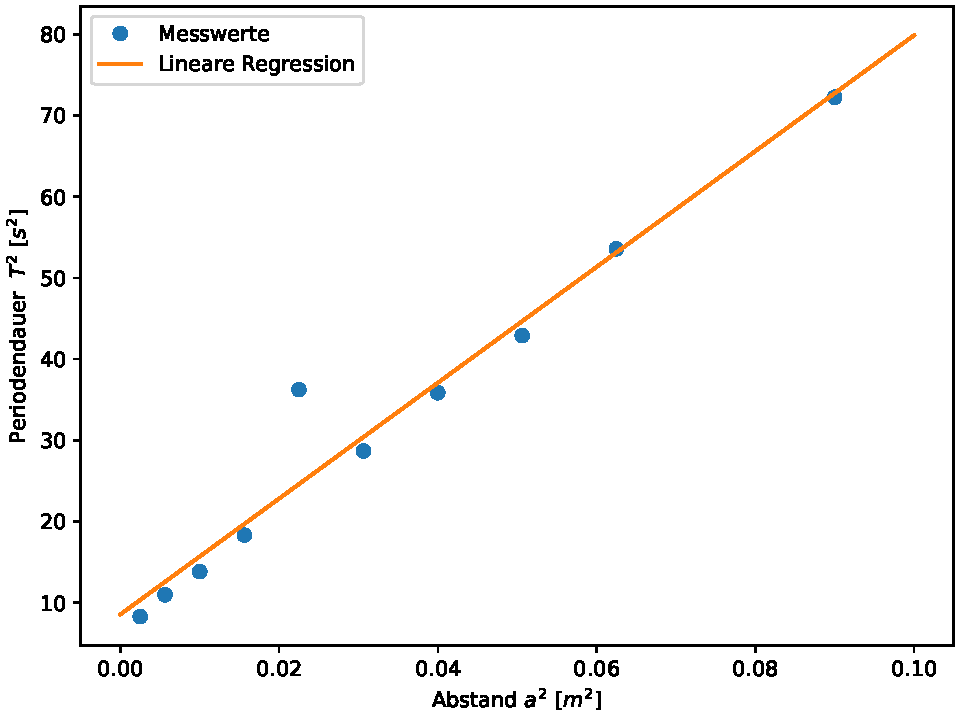
\includegraphics{plot.pdf}
    \caption{Auftragung von Periodenzeit $T^2$ gegen Abstand $a^2$}
    \label{fig:plot}
  \end{figure}

%Siehe \autoref{fig:plot}!